% Chapter 4
%
\chapter{Implementation of SendIt} % Main chapter title
%
\label{Chapter4} % For referencing the chapter elsewhere, use \ref{Chapter1} 
%
In this chapter the implementation specifics of SendIt will be discussed. It will go through how the application looks and functions, how the ACS server is implemented, and finally, how the application can be extended and improved.

\section{Application}
%
  In this section, everything regarding the implementation of the application will be discussed, except the usage modes. It will go through the implementation and usage of SendIt and clearly explain how the different concepts and technology works.
  %
  \subsection{Cryptography}
  \label{sec:crypto_imp}
    In SendIt's implementation, the Web Crypto API (SubtleCrypto module) is used for generating and handling keys \cite{ar_webcrypto}. This allows for an easy and reliable way to standardize the handling of keys, encryption and decryption, in every system. The Web Crypto API is available in most internet browsers. It has been available through the Chrome browser, since the release of version 37 \cite{url_webcr_supp}. Using a pre-developed, and tested API for SendIt's cryptographic functions allows for a more reliable system. Since the implementation of the cryptographic functions and debugging has already been done, it allows more time to be spent on developing other functionality. This is the reasoning for using the Web Crypto API.

    The system begins with creating a unique key pair, if no such key pair already exists. This check is done at the time of choosing to send or receive a file so that, if desired, the user can change to the correct identity for this connection. The key pairs used consists of two RSA-OAEP 2048 bit keys with SHA-1 hashing, but this is easy to change if the need arises. The choice of key-type was based on the recommendation of the WebCrypto API specification \cite{ar_webcrypto}.

    The key-exchange is done over the secure DataChannel created by WebRTCs PeerConnection \cite{ar_webrtc}. Once a key exchange (successful connection) has taken place, the created key pair and the other identity's public key will be written to the disk.

    SendIt imports the file into memory once a key is needed. After which it extracts the keys stored. Once the keys have been used and the communication has finished, SendIt will overwrite the existing file with the new, updated information. The file containing the keys has information exceeding just the known keys. Both the identity associated with a key, and the key itself, has to be stored.

    As discussed in \Cref{sec:crypto_des}, SendIt uses symmetric and asymmetric keys, since asymmetric keys can only encrypt small amounts of data. The maximum amount of data the asymmetric key pair mentioned previously (\emph{RSA-OAEP 2048 bit with SHA-1 hashing}) can encrypt is 214 bytes \cite{PKCSV2RSA2012}. SendIt uses an AES-GCM symmetric key, with a length of 256 bits, which allows for encryption of up to \emph{2\textsuperscript{39}-256} bytes of data \cite{ar_webcrypto}. This is well within the limits of what is necessary in SendIt. 

%
  \subsection{Connection setup}
  \label{sec:conn_set_imp}
  %Connection setup - Offer&Answer generation & Processing
    This section will explain the functionality of generating the connection information and how each endpoint processes that information in order to create the connection. SendIt implements two different ways to share the connection information, in order to create a P2P connection between two endpoints. These two modes will be explained in \Cref{Chapter5}.

    %Offer / Answer generation
    The Offer and Answer generation and processing is done as described in \Cref{sec:webrtc}. The difference from the normal usage is that they can also be encrypted before being transferred, which means they have to be decrypted before being used. The original form of the data is a JavaScript object.

    To encrypt the data, it is first turned into a string, then to an ArrayBuffer, after which it is encrypted. To decrypt the data, it is converted from a string to an array of integers. It is then converted to an Uint8Array before being decrypted. The decrypted data is also an Uint8Array, which is turned into a string, and then back into a JavaScript object. All the conversions just mentioned, stem from the different data formats required by the different libraries and frameworks. For more information on how the data is exchanged, see \Cref{Chapter5}.

    %ICE and SDP? How and waht differs?
    The actual setup of the connection and the creation of the DataChannel is done according to the examples and descriptions in \Cref{sec:webrtc}. The only difference in connection setup between the two modes, is if ICE trickling is used or not.

    When the Offer and Answer is successfully exchanged, a direct connection is created. There are scenarios, when this is not case. Known causes of issues with completing the connection are:
    %
    \begin{itemize}
      \item Setup not completed within a certain time frame (see \Cref{Chapter6})
      \item One or both endpoints are behind symmetrical NAT
      \item One or both endpoints change network location (For example, connect to a different network.)
    \end{itemize}
    %

    When implementing SendIt, the choice was made to not support symmetrical NAT, as it requires a TURN server. This means the connection would no longer be a direct end-to-end connection. 
    Widespread use of IPv6 would solve this issue, as it would eliminate the need for NAT traversal and TURN servers. As for changes in network conditions, there is nothing to be done on the application side, except including a signaling server. As such, the system assumes that users will stay in the same network conditions for the duration the connection is active. For the ACS mode, automatic reconnection is an option which can be added as an extra feature.
  
  \subsection{File transfer functionality}
    %Chunking & Size limit
    The communication will consist mostly of file data, and as such, it is interesting to know how much data can be handled. In theory, splitting files into chunks during reading, and then transferring these chunks, allows for infinitely large transfers. The default max size for Node.js is approximately 1 GB for 32-bit machines, and 2 GB for 64-bit machines. This indicates the maximum amount of data that can be kept in memory. The reason for this limit is because this is the max amount of data the V8 JavaScript engine used by Node.js can have in memory at the time \cite{url_node,url_v8}.

    The current functionality separates each file into chunks of 1200 bytes, as is the limit imposed by the Chromium implementation of WebRTC \cite{SctptransportCcCode}. The max file size is set to 160 megabytes during development, since it was the max size used by PubShare \cite{url_pubshare}. It is likely that this can be increased without any issues, since Node.js has support for keeping larger files in memory, but it would require some testing before being ready to deploy. See \Cref{fig:file_off} for an illustration of the previous explanation.

  \subsection{Programming languages, libraries and frameworks}
    SendIt is developed in JavaScript utilizing the Electron framework. These technologies were chosen because they allow for easy implementation, while supporting multiple operating systems. Easy connection setup and direct communication via P2P is also available, through pre-developed and tested frameworks. In addition, it also allows for the use of existing libraries and standardizations developed for web browsers, in desktop applications. 

    To clarify, this means that the user does not need to open their web browser to utilize SendIt, but can install it and run it like they would run any desktop program with a GUI. It also allows for easy creation of an installer file, which means the end user only needs to download and run the installer, for the program to be usable.

    %
    \begin{figure}
    \centering
    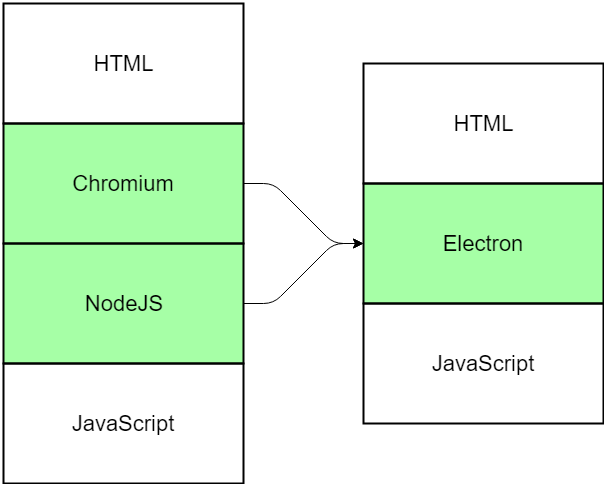
\includegraphics[width=60mm]{Dev_Stack_New}
    \caption[Application stack]{The stack for the prototype application. It is built using HTML, Electron, and JavaScript.}
    \label{fig:dev_stack}
    \end{figure}

    The electron framework uses Node.js for the back end and Chromium for the front end \cite{url_electron}. In practice, this means that the system is built on: HTML, Electron and JavaScript, where Electron utilizes Chromium and Node.js. (see \Cref{fig:dev_stack}) This allows us to use modules and frameworks from any of the previously mentioned entities independently. Our implementation uses these libraries and frameworks:
    %
    \begin{itemize}
    \item Node.js API - Used for reading and writing to the disk and finding correct files and folders \cite{url_node}.
    \item Chrome Web Cryptography API - Used to handle the creation and exportation of keys, encryption, and decryption \cite{ar_webcrypto,url_webcr_supp}.
    \item Node.js Clipboardy - Utilized to automatically copy the generated Offer/Answer to the clipboard \cite{url_clipboardy}.
    \item Node.js Electron-prompt - Used to create pop-ups for requesting user input \cite{url_ele-prompt}.
    \item Chrome Native WebRTC - Used for creating and managing WebRTC connections \cite{url_webrtc_chrome}.
    \item jQuery v3.2.1 - Utilized to manage front end actions and dynamic updates \cite{url_jQuery}.
    \item Bootstrap v3.3.7 - Used to manage front end modules and dynamic updates \cite{url_bootstrap}.
    \end{itemize}
    %

  %
  \subsection{Program flow}
  \label{sec:progflow}
  %Program Flow
  The general appearance of the program will be explained in the following section. The functionality which is unique to each mode will be discussed in \Cref{Chapter5}. That means that most of the actual functionality is not explained here, but rather the installation, setup, and settings available. In addition, it will also explain the screens not related to the connection setup. These include the waiting screen, the transfer status screen, and the transfer complete screen.
  %
    \subsubsection*{Installation and launching application}
    %Installation and launch
      %Screenshots and explanation
    The application comes in the form of installer files for Linux, Mac, and Windows. These files are in the format of \emph{.deb} for Linux, \emph{.dmg} for Mac, and \emph{.exe} for Windows. The installers are very basic and require no interaction except executing them. After that is done, the image shown in \Cref{fig:inst} will appear and display a small animation. Afterwards, SendIt is installed and will be available. In most cases, the icon will be available on the desktop. Once the application is launched for the first time, a pop-up window will appear, as indicated in \Cref{fig:popup}. Afterwards, the user is taken to the Home screen. This pop-up window will only be displayed the first time the program is opened.
    \begin{figure}[H]
      \centering
      
\includegraphics[width=60mm]{Figures/Base/installer}
      \decoRule
      \caption[SendIt: Install animation]{While the installation of SendIt is ongoing, this small box, with basic animations, will appear. Once it disappears, the program is installed.}
      \label{fig:inst}
    \end{figure}

    \begin{figure}[H]
      \centering
      
\includegraphics[width=80mm]{Figures/Base/start_up}
      \decoRule
      \caption[SendIt: First launch pop-up]{This pop-up appears the first time the program is started. It informs the user of the default location of the upload folder. The files the user wants to send should be placed in this folder.}
      \label{fig:popup}
    \end{figure}  
    %
  \subsubsection*{Home screen}
  %Home screen
    %Screenshot & explanation. Include popup!
  The Home screen is the first screen the user sees. On this screen, there is not much detail or information. The logo and acronym for SendIt is displayed, as well as the navigation bar. From here on, it is all about choosing the desired functionality or tweaking the settings to fit the users desire. The only difference between the Home screen for the two modes, is the formatting of the word 'Serverless' at the bottom of the screen, as well as the ACS mode not having a receive button on the navigation bar.
    \begin{figure}[H]
      \centering
      
\includegraphics[width=\textwidth]{Figures/Base/Home_Screen}
      \decoRule
      \caption[SendIt ACS mode: Home screen]{The Home screen displayed when the application is in ACS mode. The navigation bar has no button for receiving files. The 'Serverless'-part of SendIt's acronym is also crossed out, at the bottom of the page.}
      \label{fig:hs_acs}
    \end{figure}

    \begin{figure}[H]
      \centering
      
\includegraphics[width=\textwidth]{Figures/Base/Home_Screen_SL}
      \decoRule
      \caption[SendIt Serverless mode: Home screen]{The Home screen displayed when the application is in Serverless mode. The navigation bar has a button for both sending and receiving files.}
      \label{fig:hs_sl}
    \end{figure}

  \begin{figure}[H]
      \centering
      
\includegraphics[width=\textwidth]{Figures/Base/navbar_sl}
      \decoRule
      \caption[SendIt: Navigation bar]{The navigation bar displayed in Serverless mode. The receive-button is not present in the ACS mode, since a separate page will be displayed if someone offers to send file(s) to you. This bar is always displayed at the top of the window.}
      \label{fig:hs_nb}
    \end{figure}
  %
  \subsubsection*{Settings}
  %Settings screen
    %Screenshot and explanation.
    The base view of the settings page is represented in \Cref{fig:sett}. At the top one can input which identity (or e-mail address if you will) to use. Further down, one can remove the configuration file, the file which stores all the data about which identity and which settings to use. Following are radio buttons, where one can choose which mode to use and if one wants to use custom locations, for example, where to store downloaded files. At the bottom, information about the current settings are displayed. Finally, there is a 'save changes' button, to store the changes made.

    In \Cref{fig:set_det}, more detailed options are displayed. These appear when clicking the non-default option of the radio buttons. If the ACS option is selected for \emph{Mode selection}, the field for indicating the address of the server is displayed, as well as a 'save' button and a 'reset' button. Afterwards, there is an option for manually selecting a file from which to load keys. One can also remove the file currently used, by pressing the 'remove ALL current keys!' button or remove individual keys by clicking on the corresponding e-mail address. Finally, one can customize the download and upload folder location.
    %Base screen
    \begin{figure}[H]
      \centering
      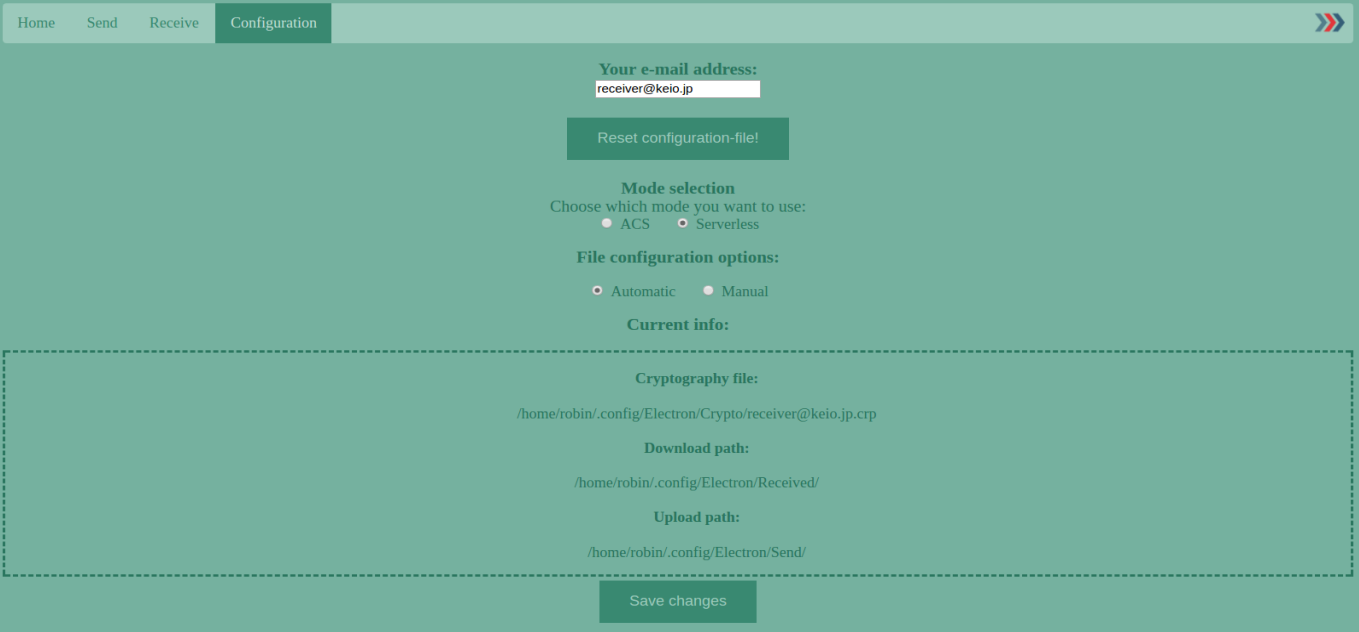
\includegraphics[width=\textwidth]{Figures/Base/Settings}
      \decoRule
      \caption[SendIt: Settings screen]{The screen used for indicating user preferences, upload and download locations, identity management, and mode selection.}
      \label{fig:sett}
    \end{figure}

    %Details screen
    \begin{figure}[H]
      \centering
      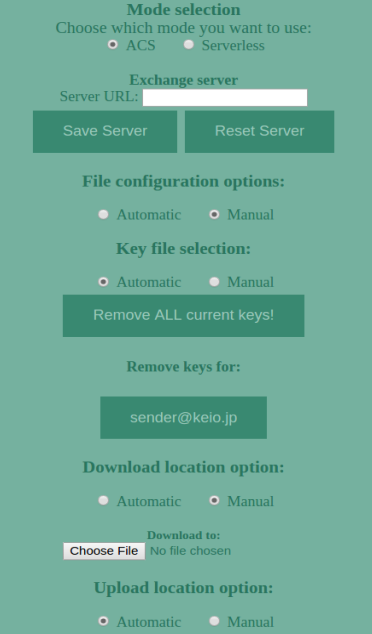
\includegraphics[width=70mm]{Figures/Base/settings_expanded}
      \decoRule
      \caption[SendIt: Detailed settings screen]{The expanded version of the settings screen with the selections and menus displayed.}
      \label{fig:set_det}
    \end{figure}

  \subsubsection*{After successful connection setup}
  \label{sec:file_recv}
  %
    All the following examples are taken from the Serverless mode, but they look identical in the ACS mode, with the exception of the navigation bar. These are the different screens shown once the endpoint has completed their part of the connection setup exchange.\\
     
    \noindent
    \underline{Waiting screen}\\
    The waiting screen is displayed while the endpoints are waiting for WebRTC to establish the P2P connection.
    \begin{figure}[H]
      \centering
      
\includegraphics[width=\textwidth]{Figures/Base/waiting}
      \decoRule
      \caption[SendIt: Waiting for connection screen]{This screen is displayed while waiting for the endpoints to connect via P2P (WebRTC).}
      \label{fig:SL_wait}
    \end{figure}

    %
    \noindent
    \underline{Transfer screen}\\
      It displays details about the current file being transferred; it's name and type, as well as the total number of files to transfer. It also shows the percentage of data transferred for the current file. Finally, there is a cancel button in case one end wants to stop the transfer.
    \begin{figure}[H]
      \centering
      
\includegraphics[width=\textwidth]{Figures/Base/transfer}
      \decoRule
      \caption[SendIt: Transfer screen]{This screen displays details about the status of the current transfer.}
      \label{fig:SL_trans}
    \end{figure}

    %
    \noindent
    \underline{Connection completed screen (\emph{Sender})}
    \begin{figure}[H]
      \centering
      
\includegraphics[width=\textwidth]{Figures/Base/sender_complete}
      \decoRule
      \caption[SendIt: Final screen (Sender)]{This screen displays details about which files were transferred.}
      \label{fig:SL_rec1}
    \end{figure}

    %
    \noindent
    \underline{Connection completed (\emph{Receiver})}
    \begin{figure}[H]
      \centering
      
\includegraphics[width=\textwidth]{Figures/Base/receiver_complete}
      \decoRule
      \caption[SendIt: Final screen (Receiver)]{This screen displays details about which files were received. It also has an 'open containing folder'-button for easy access to the received files.}
      \label{fig:SL_rec2}
    \end{figure}
%
\section{ACS server implementation}
\label{sec:acs_serv_imp}

  The ACS server is implemented in JavaScript, using the Node.js environment. It uses a library implementing the Web Crypto API for Node.js \cite{WebcryptoW3CWeb2018}, which allows for the use of the same keys, the same encryption scheme and generally the same cryptographic solutions as in the application. This makes it easy to use and means there is no need for developing support for, or using other cryptographic methods, to authenticate with the ACS server.

  \subsection{WebSockets}
  \label{sec:acsws}
  %WS
    %How is it used, secure, advantage
    %IMPLEMENTATION
    All communication between endpoints and the ACS server is done over WebSockets using HTTPS. This enables bi-directional communication at any time and creates an easy interface to use for communicating with different endpoints. The communication is exclusively done using the protocol described in the next section.
    
    The WebSocket interface and API also allows for easy handling and management of clients. Clients can connect and disconnect randomly without affecting the service as a whole. All clients are treated equally and it is easy to address each client individually. Because of this, it is very easy to receive information from one client and immediately forward it to the intended recipient. 

  \subsection{Protocol}
  \label{sec:prot_imp}
  This section reviews the implementation of the protocol discussed in \Cref{sec:wsprot}. For an overview of the packet format, see \Cref{tab:basic}. The format indicated for each of these packets, goes in the data field of the general packet format. Following is the practical implementation of the protocol.
  %
  \subsubsection*{Lookup}
 %
  The \emph{Lookup} packet from client to server does not contain any data. The packet sent from the server to the client can contain the data indicated in \Cref{tab:lookup}. If \emph{res} is \emph{true}, the data will consist of the fields \emph{res}, \emph{wrap} and \emph{key}. The \emph{wrap} field consist of the symmetric key, encrypted with the other endpoint's public key. If \emph{false}, it will consist of \emph{res} and \emph{key} only.
%
  \begin{table}
    \caption[ACS protocol: Lookup packet]{Lookup packet}
    \label{tab:lookup}
    \centering
    \begin{tabular}{l l l l}
      \tabhead{Name} & \tabhead{Type} & \tabhead{Argument details} & \tabhead{Required} \\
      \midrule
      res & Boolean & Indicates if authentication setup is needed or not & Yes\\
      key & JWK & Server's public key in JWK format & Yes\\
      wrap & Array & Encrypted symmetric key& No\\
      \bottomrule\\
    \end{tabular}
  \end{table}
%
  \subsubsection*{Authentication setup}
  %
  The possible arguments used by the Authentication setup and Authentication Setup Reply functionality are shown in respectively \Cref{tab:auth_set} and \Cref{tab:auth_s_r}. The public key of the client is sent to the server. The server tries to set up authentication for subsequent connections. The authentication setup is considered a success if no previous data is stored for this e-mail or public key. If this is the case, the \emph{Authentication Setup Reply} packet will contain \emph{res} and \emph{wrap}, where \emph{res} is set to \emph{true}. The \emph{wrap} field consists of the symmetric key, encrypted with the other endpoint's public key. If the setup fails, the \emph{wrap} field is not included.
%
  \begin{table}
    \caption[ACS protocol: Authentication Setup packet]{Authentication Setup packet}
    \label{tab:auth_set}
    \centering
    \begin{tabular}{l l l l}
      \tabhead{Name} & \tabhead{Type} & \tabhead{Argument details} & \tabhead{Required} \\
      \midrule
      key & JWK & Client's public key in JWK format & Yes\\
      \bottomrule\\
    \end{tabular}
  \end{table}
%
  \begin{table}
    \caption[ACS protocol: Authentication Setup Reply packet]{Authentication Setup Reply packet}
    \label{tab:auth_s_r}
    \centering
    \begin{tabular}{l l l l}
      \tabhead{Name} & \tabhead{Type} & \tabhead{Argument details} & \tabhead{Required} \\
      \midrule
      res & Boolean & Authentication result & Yes\\
      wrap & Array & Encrypted symmetric key& No\\
      \bottomrule\\
    \end{tabular}
  \end{table}
%
  \subsubsection*{Authentication}
  %
  \Cref{tab:prot_auth} and \Cref{tab:prot_auth_rep} shows the possible arguments for the authentication packets. The \emph{ciph} field contains the client's email address, encrypted with the symmetric key. The \emph{Authentication Result} packet returns a boolean value directly in the data field, indicating the result of the authentication process. Successful authentication returns \emph{true}.
%
  \begin{table}
    \caption[ACS protocol: Authentication packet]{Authentication packet}
    \label{tab:prot_auth}
    \centering
    \begin{tabular}{l l l l}
      \tabhead{Name} & \tabhead{Type} & \tabhead{Argument details} & \tabhead{Required} \\
      \midrule
      ciph & Array & Client's encrypted e-mail address & Yes\\
      \bottomrule\\
    \end{tabular}
  \end{table}
%
  \begin{table}
    \caption[ACS protocol: Authentication Result packet]{Authentication Result packet}
    \label{tab:prot_auth_rep}
    \centering
    \begin{tabular}{l l l l}
      \tabhead{Name} & \tabhead{Type} & \tabhead{Argument details} & \tabhead{Required} \\
      \midrule
      - & Boolean & Authentication result & Yes\\
      \bottomrule\\
    \end{tabular}
  \end{table}
 % 
  \subsubsection*{Init}
  %
  The \emph{Init} packet can consist of the data shown in \Cref{tab:init}. It contains information about the files being offered. Each object in the \emph{files} array has information about the file name, file type and the size of the file.

   \begin{table}
    \caption[ACS protocol: Initiate Connection packet]{Initiate Connection packet}
    \label{tab:init}
    \centering
    \begin{tabular}{l l l l}
      \tabhead{Name} & \tabhead{Type} & \tabhead{Argument details} & \tabhead{Required} \\
      \midrule
      files & Array & Array of objects with file data & Yes\\
      \bottomrule\\
    \end{tabular}
  \end{table}
%
  \subsubsection*{Accept}
  %
  The \emph{Accept} packet contains the WebRTC Offer generated and indicates that the endpoint wants to receive the data previously offered. The WebRTC Offer can either be encrypted or in cleartext. See \Cref{tab:acc} for more information about the data transferred. If the Offer is sent in cleartext, the data transferred is just the WebRTC Offer object. If not, the data consists of the other three fields (\emph{wrap}, \emph{iv}, and \emph{ciph}). The \emph{wrap} field consists of the symmetric key, encrypted with the other endpoint's public key. The \emph{ciph} field consists of the WebRTC Offer, encrypted with the symmetric key.

  \begin{table}
    \caption[ACS protocol: Accept packet]{Accept packet}
    \label{tab:acc}
    \centering
    \begin{tabular}{l l l l}
      \tabhead{Name} & \tabhead{Type} & \tabhead{Argument details} & \tabhead{Required} \\
      \midrule
      - & Object & The WebRTC Offer generated by the endpoint & No\\
      wrap & Array & Encrypted symmetric key & No\\
      iv & Array & Initialization vector for the symmetric key & No\\
      ciph & Array & Encrypted WebRTC Offer & No\\
      \bottomrule\\
    \end{tabular}
  \end{table}
  %
  \subsubsection*{Refuse}
  The refuse packet contains no data. If this packet is received the connection setup is stopped.
%
  \subsubsection*{Answer}
%
 The \emph{Answer} packet contains the WebRTC Answer generated by the endpoint. The WebRTC Answer can either be encrypted or in cleartext. See \Cref{tab:ans} for more information about the data transferred. If the Answer is sent in cleartext, the data transferred is just the WebRTC Answer object. If not, the data consists of the other two fields (\emph{iv} and \emph{ciph}). The \emph{iv} field consists of the initialization vector, encrypted with the other endpoint's public key. The \emph{ciph} field consists of the WebRTC Answer, encrypted with the symmetric key.
 %
\begin{table}
    \caption[ACS protocol: Answer packet]{Answer packet}
    \label{tab:ans}
    \centering
    \begin{tabular}{l l l l}
      \tabhead{Name} & \tabhead{Type} & \tabhead{Argument details} & \tabhead{Required} \\
      \midrule
      - & Object & The WebRTC Answer generated by the endpoint & No\\
      iv & Array & Encrypted initialization vector for the symmetric key & No\\
      ciph & Array & Encrypted WebRTC Answer & No\\
      \bottomrule\\
    \end{tabular}
  \end{table}
%
  \subsubsection*{ICE}
%
  This packet contains the data showed in \Cref{tab:ice}. The data can either be encrypted or sent in cleartext. If it is not encrypted, it will be sent as an ICE candidate object. If it is encrypted, it will consist of the fields \emph{ciph} and \emph{iv}. The \emph{ciph} field consists of the ICE candidate, encrypted with the symmetric key.
%
  \begin{table}
    \caption[ACS protocol: ICE packet]{ICE packet}
    \label{tab:ice}
    \centering
    \begin{tabular}{l l l l}
      \tabhead{Name} & \tabhead{Type} & \tabhead{Argument details} & \tabhead{Required} \\
      \midrule
      - & Object & The ICE candidate generated by the endpoint & No\\
      ciph & Array & Encrypted ICE candidate & No\\
      iv & Array & Initialization vector for the symmetric key & No\\
      \bottomrule\\
    \end{tabular}
  \end{table}
%
  \subsubsection*{Done}
%
  The \emph{done} packet contains no data, and indicates that the connection is terminated and that the endpoints are ready for a new connection.
%
  \subsubsection*{Error}
%
  The \emph{error} packet can contain data about which error occurred. If the server receives an \emph{error} packet with an indicated destination, it will forward it to the correct endpoint. The data will have the format indicated in \Cref{tab:err}.
%
  \begin{table}
    \caption[ACS protocol: Error packet]{Error packet}
    \label{tab:err}
    \centering
    \begin{tabular}{l l l l}
      \tabhead{Name} & \tabhead{Type} & \tabhead{Argument details} & \tabhead{Required} \\
      \midrule
      - & String & Error details & No\\
      \bottomrule\\
    \end{tabular}
  \end{table}
%
  \subsubsection*{Wait}
%
  The \emph{wait} packet does not contain data. It indicates that an endpoint is busy, and, as such, cannot partake in a connection at this time. If a destination is specified, the server forwards the packet to the correct endpoint.
%
\section{Extendability and improvements}
%
In this section the extendability of SendIt, in general, will be assessed. SendIt can be used as a platform to build extended functionality, and as such, it should be noted in what way this can be done, and how one stands to benefit from doing it. It will also discuss possibilities for improving the current implementation.

  \subsection{Key storage encryption}
  %
    The file where keys are stored should be encrypted and password protected, or otherwise access restricted. The key file should only be usable if the correct password is provided. If the wrong password is provided, the keys should not be accessible. The key file should be updated every time it is used by the system. This will allow users to change the password used to access the keys between each use and also make it easy to update information regarding each key. In addition, it gives no guarantee that the same encryption is used each time, which makes attacks over time harder to execute, since there is no reliable way to analyze changes or patterns in the way the file is stored. This functionality should be implemented and would improve the solution. It is not currently implemented in SendIt, due to time constraints. 

  \subsection{E-mail verification}
  %E-mail verification
    One way to extend the current functionality is to add e-mail verification to the process of registering an identity. This would increase the trustworthiness of each identity since proving ownership of the registered e-mail address would be a necessity. It would however, also include all the issues stemming from how the e-mail system is implemented. It would also make the registration process harder and require more from the users before being able to use the system. Because of these issues, it is not included in the system by default, but can easily be added. It is left up to the end users to develop and extend the proposed system, if such functionality is desired.

  \subsection{Support for bigger files}
  \label{sec:bigfile}
  %
    Supporting bigger files can be achieved by reading in chunks of the file. Then, once a chunk is completely transferred, the next chunk is read into memory. This will allow both endpoints to handle smaller amounts of data at a time, while still having transmitted the whole file after the transfer of all chunks have been completed. It is not recommended to implement this until after the 'resume transfer' feature is implemented, as transferring large amounts of data, without any way of resuming it in case of failure, is less than optimal.

  \subsection{Resume transfer}
  \label{sec:res_trans}
    %
    \begin{table}
      \caption[Record of communication]{Fields included in the record of communication.}
      \label{tab:comm_rec}
      \centering
      \begin{tabular}{cccc}
            \textbf{Sender} & \textbf{File(s)} & \textbf{Date} & Completed \\
            \midrule
            test@email.com & picture.jpg & 2018-03-20 & 0\\
            another@email.com & document.doc & 2018-05-13 & 4\\
            \bottomrule
      \end{tabular}\\
    \end{table}
    %
    This functionality can easily be implemented based on a communication record. Since every identity will have a list of previously transferred files, it will have the file name included. If the transfer is not completed, this record can store information about which chunk of the file was the last to be received, and the endpoint can request the transfer to be continued from there.

    If the sender is not willing to resume the previous transfer, it can either start over, or the sender can offer to transfer another file. This decision is up to the sender's settings and/or preference. If the sender choses to not resume the transfer, the data previously stored on the receiver's local system should be removed, and the record updated as a failed transfer. The system should only allow for the requested file to be shared on the subsequent connection. 

    To clarify: Alice tries to send Bob \emph{File A}, but the connection is broken. If Alice tries to send \emph{File A} again, it will resume from the last chunk received. If it fails again, it will also allow for the transmission of \emph{File A} to be resumed. However, if Alice contacts Bob again, but tries to send \emph{File B} this time, the previously transmitted information (\emph{File A}) stored by Bob should be removed.

    The record of communications can be implemented by creating a log that contains the fields indicated in \Cref{tab:comm_rec}. The last field can either be \emph{-1} (meaning failed), \emph{0} (meaning success) or the number of the last received chunk. This is useful for being in compliance with the GDPR, allowing the user to keep track of their interactions for reviewing their activity, and implementing a 'resume transfer' functionality, as mentioned.

  \subsection{WebRTC IDP inclusion}
  %WebRTC IDP
    WebRTC comes with a suggested standard for implementing Identity Provider services. An Identity Provider is a trusted third party that corroborates an identity. An example would be connecting ones Facebook account to an identity, as a means for other endpoints to verify the authenticity of that identity. This is possible for many different services and can be a means of increasing trust in identities. Currently, there are some arguments and disagreements on how this should be implemented in WebRTC, and as such, there are very few existing frameworks that can be used. This is expected to change, and at that point, using these services will allow for an easier way to increase trust in endpoints.

    The trust is of course reliant on the end user already trusting the service that is used as the Identity Provider, and that the identity is as expected. For example:\\
    If the Identity Provider used is a known service (such as Facebook), one can reasonably trust the data received. If it is from a service unknown to the user, then the identity provision does not increase the trust at all, since the data may be created for malicious purposes. In the same way, if the endpoint is expecting to be communicating with Alice, but Bob's identity is asserted by the provider, the end user should be sceptical.

    In summary, this functionality would allow one to link accounts from other, independent services with their WebRTC connection, in order to corroborate the endpoint's identity and increase trust.

  \subsection{SendIt as a platform}
  %
    This is an interesting idea since the proposed system allows for connection setup and identity assertion. One can use SendIt for this functionality and build any kind of additional functionality on top, if so desired. Especially combining with VOIP, which WebRTC is often used for, can be useful. It allows the developers to focus on their services and additional functionality, while allowing the easy to use and secure setup offered by SendIt to take care of identity management and authentication. The design and implementation of SendIt is modular, which means one can easily pick and choose which functionality one wants to utilize, and discard the rest. This makes it easy to take advantage of the wanted functionality, while not complicating the solution by including the functionality that is not useful to the specific scenario at hand. 